\documentclass[11pt]{article}
\usepackage[margin=1in]{geometry}
\usepackage{amsmath,amssymb,amsthm,mathtools,bm}
\usepackage{booktabs,tabularx,array,longtable}
\usepackage{graphicx}
\usepackage{xcolor}
\usepackage{microtype}
\usepackage{enumitem}
\usepackage{caption}
\usepackage{subcaption}
\usepackage{float}
\usepackage{siunitx}
\usepackage{hyperref}
\usepackage[nameinlink,capitalise]{cleveref}
\graphicspath{{search/results/figures/}{learning/figures/}}
\hypersetup{colorlinks=true,linkcolor=blue!55!black,citecolor=green!35!black,urlcolor=blue!55!black}
\setlist{nosep}
\newtheorem{theorem}{Theorem}[section]
\newtheorem{proposition}[theorem]{Proposition}
\newtheorem{corollary}[theorem]{Corollary}
\newtheorem{lemma}[theorem]{Lemma}
\theoremstyle{definition}
\newtheorem{definition}[theorem]{Definition}
\newtheorem{example}[theorem]{Example}
\theoremstyle{remark}
\newtheorem{remark}[theorem]{Remark}
\newcommand{\cH}{\mathcal H}
\newcommand{\cE}{\mathcal E}
\newcommand{\cJ}{\mathcal J}
\newcommand{\cU}{\mathcal U}
\newcommand{\cA}{\mathcal A}
\newcommand{\Tr}{\operatorname{Tr}}
\newcommand{\rank}{\operatorname{rank}}
\newcommand{\id}{\operatorname{id}}
\newcommand{\R}{\mathbb R}
\newcommand{\C}{\mathbb C}
\newcommand{\Z}{\mathbb Z}
\newcommand{\JS}{\operatorname{JS}}
\newcommand{\TV}{\operatorname{TV}}
\title{\textbf{Covariant Quantum Memory and Emergent Goal Geometry}\\
\large Exact Qutrit Torus Metrics, Predictive Fibers, and Opaque Action Learning}
\author{Quantum Hodology Research Project}
\date{\today}
\begin{document}
\maketitle

\begin{abstract}
We ask whether a three-dimensional quantum system can support an
operationally learned two-dimensional space when action meanings are inferred
from future observations rather than supplied as coordinate labels. The
construction uses Weyl-covariant qutrit instruments on the nine Hesse
symmetric informationally complete states. A correction of terminal semantics
is decisive. If success means that the current predictive state has reached
the goal, the original integrated Hesse instrument has exact Bellman shells
\[
V_{\rm self}=0,\qquad V_{\rm edge}=4,\qquad V_{\rm diagonal}=5.
\]
This is a nondegenerate translation-invariant metric on \(\Z_3^2\). The
earlier shells \(4,4,5\) answer the different report-the-goal-again task and
are nonmetric. We prove a general theorem under which positive covariant
hitting costs form a group metric and derive the exact Schoenberg spectrum of
the Hesse metric: it is Euclidean of minimal rank eight, so it recovers a
two-dimensional torus topology but not a global planar embedding.

We introduce an exactly soluble integrated family with an observed unitary
memory branch and informative Hesse reset branches. For sharp reports its
Bellman shells are
\[
E=\frac4{(1+\mu)^2},\qquad
D=\frac{3\mu+5}{(1+\mu)^2}.
\]
It continuously interpolates between informative reset geometry and the
exact torus word metric. The analytic value
\(\mu=(4\sqrt2-5)/3\) makes every elementary cell an exact Euclidean square.
A deterministic 380-point search selects \((\mu,\xi)=(0.8,1)\) as a
high-memory compromise: \(0.050326\) bits of immediate information, shells
\((0,1.234568,2.283951)\), and \(3.33\%\) scaled distortion from torus word
distance. Oracle-labelled trials identify this exact family's finite action
maps; a separate opaque Lüders experiment recovers the order-nine commuting
translation group from emitted strings.

For the outcome-discarded channel, equal-length paths with the same displacement
close exactly, while cancelling detours accumulate different noise. That noise
age is not an extra state for an agent observing every branch: its conditional
state remains a Hesse ray. Separate Lüders-instrument experiments confirm
latent future-predictive memory while showing that naive finite suffix models
do not learn it reliably. We therefore find a candidate fiber, not an already
learned bundle. We state
reproducible acceptance criteria for larger tori, local flat patches, and
spectral predictive-state learning.
\end{abstract}
\tableofcontents

\section{Motivation: geometry from attainable goals}

Quantum hodology asks whether spatial distance can be reconstructed from an
agent's goal-directed behavior. A goal reached cheaply and reliably is near;
one requiring long, risky, or costly intervention is far. If optimal goal
costs organize themselves into a low-dimensional homogeneous geometry, an
agent's controlled trajectory may be interpreted as motion in emergent space.

This requires more than plotting assigned state labels. A convincing
construction must answer three separate questions:
\begin{enumerate}
\item Can the agent distinguish predictive situations using future
statistics?
\item Can it learn what opaque actions do without coordinate names?
\item Do optimal goal costs satisfy the axioms and local structure of the
claimed geometry?
\end{enumerate}
A classical counter can trace a grid even when quantum observations contain
no corresponding structure. Conversely, quantum actions can be
distinguishable without forming translations.

The present study retains quantum state across selected observed branches.
This suggests a future base/fiber geometry: the base records place-like
translation on a finite torus, while a fiber could record purity, posterior
phase, or hidden memory. In the exact observed-branch family, nonselective
noise age appears only when outcomes are discarded. It also forces an honest distinction between global
torus topology and a locally flat planar patch.

\paragraph{Contributions.}
\begin{itemize}
\item First-principles controlled-instrument and predictive semantics.
\item An exact terminal-semantics correction and proof of Hesse shells
\((0,4,5)\).
\item A general covariant hitting-cost metric theorem.
\item Exact Fourier--Schoenberg classification of the global metric.
\item Two retained-memory constructions: an exactly finite observed
memory/reset family and a Lüders-like latent-memory family.
\item Closed-form Bellman values, an analytic local-square point, numerical
search, opaque learning, controls, and a larger-torus program.
\end{itemize}

\section{Controlled quantum processes}

\subsection{States, channels, and instruments}

Let \(\cH\simeq\C^3\). A density operator satisfies
\(\rho\succeq0\), \(\Tr\rho=1\). For action \(a\in\cA\), an instrument is
\[
\mathfrak I^a=\{\cE_o^a:o\in\mathcal O\}
\]
where each branch is completely positive and trace nonincreasing and
\(\Phi_a=\sum_o\cE_o^a\) is trace preserving
\cite{Kraus1983,NielsenChuang2010}. A Kraus representation is
\[
\cE_o^a(\rho)=\sum_\alpha K_{a,o,\alpha}\rho
K_{a,o,\alpha}^\dagger,\qquad
\sum_{o,\alpha}K_{a,o,\alpha}^\dagger K_{a,o,\alpha}=I.
\]
The outcome and posterior are
\[
p(o\mid\rho,a)=\Tr\cE_o^a(\rho),\qquad
\rho_{a,o}=\frac{\cE_o^a(\rho)}{p(o\mid\rho,a)}.
\]

Several ranks are distinct. Hilbert dimension counts amplitudes. Branch Choi
rank counts minimal Kraus operators. Matrix rank of a Kraus operator controls
invertibility on state support. Predictive Hankel rank measures
future-statistical dimension. Schoenberg rank measures Euclidean embedding
dimension.

\subsection{Histories, tests, and predictive equivalence}

A history \(h=(a_1,o_1)\cdots(a_t,o_t)\) has unnormalized state
\[
\widetilde\rho_h=
\cE_{o_t}^{a_t}\circ\cdots\circ\cE_{o_1}^{a_1}(\rho_0).
\]
A future test \(\tau=(b_1,y_1)\cdots(b_k,y_k)\) has probability
\[
p(\tau\mid h)=
\frac{\Tr[
\cE_{y_k}^{b_k}\circ\cdots\circ\cE_{y_1}^{b_1}
(\widetilde\rho_h)]}{\Tr\widetilde\rho_h}.
\]
The controlled Hankel matrix \(H_{h,\tau}=p(\tau\mid h)\) contains all
operational predictions.

\begin{definition}[Predictive equivalence]
Histories \(h,h'\) satisfy \(h\sim h'\) when
\[
p(\tau\mid h)=p(\tau\mid h')
\]
for every admissible future test. Their classes are causal or predictive
states.
\end{definition}

A predictive-state representation stores probabilities of core tests instead
of a privileged density matrix. When the Hankel rank is \(r\), \(r\)
independent core predictions suffice \cite{Littman2001}. A qutrit density
operator occupies an eight-dimensional affine space, but restricted controls
may lower predictive rank, while a classical memory register may raise total
history dimension.

\subsection{Action meaning and gauge}

An action's operational meaning is its transformation of future
probabilities. Actions \(a,b\) are distinguishable when some history, current
outcome, and continuation test satisfy
\[
p(o,\tau\mid h,a)\ne p(o,\tau\mid h,b).
\]
Immediate mutual information may vanish although a future probe separates the
post-action states.

PSR coordinates admit invertible similarity gauges. Tokens may be permuted;
generators of \(\Z_m^2\) may be exchanged, inverted, or transformed by a
group automorphism. Gate-set tomography obeys the same principle
\cite{NielsenGST2020,DiMatteo2020}. We therefore evaluate group order,
commutation, orbit size, and held-out likelihood before privileged alignment.

\section{Covariance and predictive closure}

\subsection{Covariant instruments}

Let \(G=\Z_m\times\Z_m\), and let \(g\mapsto U_g\) be a possibly projective
unitary representation. A base instrument is covariant when
\[
\cJ_{o+g}(U_g\rho U_g^\dagger)
=U_g\cJ_o(\rho)U_g^\dagger.
\tag{3.1}
\]
Integrated actions take the form
\[
\cE_o^a=\cJ_o\circ\operatorname{Ad}_{U_a}.
\tag{3.2}
\]
Covariance gives
\[
p(o+g\mid U_g\rho U_g^\dagger,a)=p(o\mid\rho,a),
\]
so absolute labels can be shuffled while relative responses survive.

\begin{proposition}[Positive Choi-seed parametrization]
\label{prop:choi}
Let \(R_g=U_g\otimes\overline{U_g}\) act on output--input Choi space. Choose
\(C_0\succeq0\), and put \(C_o=R_oC_0R_o^\dagger\). If
\[
\Tr_{\rm out}\sum_oC_o=I,
\]
the corresponding maps form a CPTP covariant instrument. Conversely, every
transitive covariant instrument has this orbit form, with \(C_0\) invariant
under the reference outcome's stabilizer.
\end{proposition}
\begin{proof}
Unitary conjugation preserves Choi positivity. The partial-trace condition is
trace preservation of the sum. Conjugation by \(R_g\) maps \(C_o\) to
\(C_{o+g}\), proving covariance. Conversely, covariance transports a
reference Choi matrix around its orbit; independence of orbit representative
is stabilizer invariance.
\end{proof}

Writing \(C_0=LL^\dagger\) is a practical optimization parametrization:
complete positivity and covariance remain exact, while normalization is a
linear constraint.

\subsection{Nonselective path closure and a prospective fiber}

Let \(\Phi=\sum_o\cJ_o\). Covariance implies
\[
\Phi\operatorname{Ad}_{U_g}=
\operatorname{Ad}_{U_g}\Phi.
\]
For \(\Phi_a=\Phi\operatorname{Ad}_{U_a}\),
\begin{equation}
\Phi_{a_t}\cdots\Phi_{a_1}
=\Phi^t\operatorname{Ad}_{U_{a_1+\cdots+a_t}}.
\label{eq:path}
\end{equation}
Thus equal-length words with equal displacement have equal nonselective
evolution. Different lengths retain different powers of \(\Phi\), unless it
is predictively invisible or idempotent. A cancelling detour may return to the
same base point but alter the outcome-discarded ensemble. This is a
coarse-grained coordinate, not part of the fully observed conditional state.

For a finite separating battery, define
\[
\epsilon_{\rm path}(L)=
\max_{\substack{|w|,|w'|\le L\\\Delta(w)=\Delta(w')}}
\max_{h,\tau}|p(\tau\mid h,w)-p(\tau\mid h,w')|.
\]
Zero is path closure on the tested predictive quotient. Equal-length and
all-length residuals must be reported separately.

\section{The Hesse SIC and Weyl translations}

\subsection{Nine nonorthogonal landmarks in a qutrit}

Let \(\omega=e^{2\pi i/3}\), with
\[
X|j\rangle=|j+1\bmod3\rangle,\qquad
Z|j\rangle=\omega^j|j\rangle.
\]
They obey \(ZX=\omega XZ\). Although the vector representation is projective,
global phases disappear under conjugation, so
\(\operatorname{Ad}_X\) and \(\operatorname{Ad}_Z\) commute.

From
\[
|\psi_{00}\rangle=\frac{(0,1,-1)^T}{\sqrt2},
\]
define
\[
|\psi_{mn}\rangle=X^mZ^n|\psi_{00}\rangle,\qquad
\Pi_{mn}=|\psi_{mn}\rangle\langle\psi_{mn}|.
\]
Direct calculation yields the Hesse SIC identities
\begin{equation}
\frac13\sum_s\Pi_s=I,\qquad
\Tr(\Pi_s\Pi_t)=
\begin{cases}
1,&s=t,\\
1/4,&s\ne t.
\end{cases}
\label{eq:sic}
\end{equation}
Thus a qutrit supports nine operational landmarks without nine mutually
orthogonal basis states \cite{Renes2004}.

Let
\[
\cA=\{I,X,X^\dagger,Z,Z^\dagger\}.
\]
Conjugation permutes SIC projectors:
\[
U_a\Pi_sU_a^\dagger=\Pi_{s+a}.
\]
The four nontrivial actions are cardinal generators of the
\(3\times3\) Cayley torus.

\subsection{Integrated Hesse measure-and-prepare branches}

Define
\begin{equation}
K_o^{(a)}=\frac1{\sqrt3}\Pi_oU_a,\qquad
\cE_o^a(\rho)=K_o^{(a)}\rho K_o^{(a)\dagger}.
\label{eq:hesse-inst}
\end{equation}
Completeness follows from \cref{eq:sic}:
\[
\sum_oK_o^{(a)\dagger}K_o^{(a)}=
U_a^\dagger\left(\frac13\sum_o\Pi_o\right)U_a=I.
\]
For input \(\Pi_s\),
\begin{equation}
p_a(o\mid s)=
\begin{cases}
1/3,&o=s+a,\\
1/12,&o\ne s+a,
\end{cases}
\qquad \rho_{a,o}=\Pi_o.
\label{eq:hesse-law}
\end{equation}
The likelihood peak translates, while the outcome becomes the next state.
The last token is an exact predictive sufficient statistic.

For a uniform prior, the outcome marginal is uniform and immediate
information is
\[
I_{\rm Hesse}=\log_2 9-
H\left(\frac13,\underbrace{\frac1{12},\ldots,\frac1{12}}_8\right)
=0.2516291674\ {\rm bits}.
\]

\section{Terminal semantics and exact Bellman geometry}

\subsection{Two different goals}

Reinforcement learning assigns meaning to states only relative to rewards,
costs, and termination \cite{SuttonBarto2018,Puterman1994}. Here each
nonterminal intervention costs one. Two superficially similar tasks differ:
\begin{description}
\item[Report again.] Even at \(g\), the agent must act and obtain outcome
\(g\). This asks for external recertification and gives shells \((4,4,5)\).
\item[State hitting.] The episode ends when the current predictive state is
\(g\), so \(V_g(g)=0\). This asks the agent to occupy the goal state.
\end{description}
The earlier self--edge no-go was correct for report-again semantics, but it is
not a no-go for state-hitting hodology.

\subsection{Exact Hesse hitting values}

\begin{theorem}[State-hitting Hesse shells]
\label{thm:hesse}
For the instrument \cref{eq:hesse-inst}, unit action cost, and the boundary
\(V_g(g)=0\), the optimal values are
\[
\boxed{v_0=0,\qquad v_1=4,\qquad v_2=5,}
\]
where shells are torus word distances zero, one, and two from \(g\).
\end{theorem}
\begin{proof}
Symmetry reduces nine states to three shells. The goal boundary gives
\(v_0=0\). From an edge, move its likelihood peak to \(g\). The success
probability is \(1/3\). The four edge and four diagonal failure outcomes each
have probability \(1/12\), so
\[
v_1=1+\frac13v_1+\frac13v_2.
\tag{5.1}
\]
From a diagonal state, a cardinal move peaks at an edge. The off-peak goal
outcome has probability \(1/12\). The peak and three other edge outcomes
contribute \(1/3+3/12=7/12\); four diagonal outcomes contribute \(1/3\).
Thus
\[
v_2=1+\frac7{12}v_1+\frac13v_2.
\tag{5.2}
\]
Solving gives \(v_1=4,v_2=5\). Direct comparison of the five action rows
verifies the minimizing actions.
\end{proof}

\begin{corollary}
The directed hitting cost \(D(s,g)=V_g(s)\) is a
translation-invariant metric on \(\Z_3^2\).
\end{corollary}
\begin{proof}
Translation covariance and inverse controls give symmetry. Off-diagonal
values are positive. The only nontrivial triangle inequality is
\(5\le4+4\).
\end{proof}

\subsection{A general metric theorem}

\begin{theorem}[Covariant hitting costs induce a group metric]
\label{thm:metric}
Consider a controlled Markov process on a finite group \(G\). Assume:
\begin{enumerate}
\item transition laws are translation covariant;
\item every nonterminal action costs at least \(c_{\min}>0\);
\item each goal can be reached under a proper policy;
\item every policy has an equal-cost inverse-reflected policy;
\item \(V_g(g)=0\) is an absorbing hitting boundary.
\end{enumerate}
Then \(D(s,g)=V_g(s)\) is a translation-invariant metric on \(G\).
\end{theorem}
\begin{proof}
Nonnegativity is immediate. If \(s\ne g\), any successful trajectory pays at
least \(c_{\min}\), establishing strictness. Translation covariance gives
\(V_g(s)=v(g-s)\), while inverse reflection gives symmetry. Concatenate an
\(\varepsilon\)-optimal policy from \(s\) to \(u\) with one from \(u\) to
\(g\). The strong Markov property at the hitting time of \(u\) gives
\[
V_g(s)\le V_u(s)+V_g(u)+2\varepsilon.
\]
Let \(\varepsilon\downarrow0\) to obtain the triangle inequality.
\end{proof}

\begin{remark}
This proves metricity, not two-dimensional Euclidean embeddability. It also
depends essentially on state hitting. Under report-again semantics, if an
edge's aligning action has the same complete outcome/posterior kernel and cost
as an action at the goal, their Bellman right-hand sides coincide and the
self--edge collapse returns, regardless of branch Choi rank.
\end{remark}

\section{Global torus metric versus a local plane}

\subsection{Schoenberg's exact Euclidean criterion}

For a finite symmetric distance matrix \(D\), define
\[
J=I-\frac1n\bm1\bm1^T,\qquad
B=-\frac12J(D^{\circ2})J.
\]
Schoenberg's theorem states that \(D\) is a Euclidean distance matrix in
\(\R^k\) exactly when \(B\succeq0\) and \(\rank B\le k\)
\cite{Schoenberg1935}. If \(B=Q\Lambda Q^T\succeq0\), coordinates are
\(Q\Lambda^{1/2}\). Negative eigenvalues disprove exact Euclidean
embeddability; retaining two positive eigenvalues gives classical
multidimensional scaling (MDS), not an exact proof \cite{BorgGroenen2005}.

\begin{proposition}[Schoenberg spectrum of the Hesse hitting metric]
\label{prop:spectrum}
The distance \(0,4,5\) is Euclidean, but its minimal embedding dimension is
eight. Its centered Gram eigenvalues are
\[
0,\quad
\underbrace{17,\ldots,17}_{4},\quad
\underbrace{\frac72,\ldots,\frac72}_{4}.
\]
\end{proposition}
\begin{proof}
\(D^2\) is \(16\) on four cardinal displacements and \(25\) on four
diagonals. For a character \((k,l)\in\Z_3^2\), define
\(A_0=2\), \(A_1=A_2=-1\). The Fourier eigenvalue of \(D^2\) is
\[
\widehat{D^2}(k,l)=16(A_k+A_l)+25A_kA_l.
\]
For nontrivial characters with exactly one zero coordinate this is \(-34\);
when both coordinates are nonzero it is \(-7\). On the centered subspace,
\(B\) has minus one half these eigenvalues. All eight are positive.
\end{proof}

The group and neighbor graph are two-dimensional, but the global intrinsic
metric is not a planar \(3\times3\) patch. Periodic boundary points are
neighbors. This is a topology/embedding distinction, not a failure of the
torus interpretation.

\subsection{Local flatness}

For a larger \(m\times m\) torus, graph balls of radius \(r<m/2\) lift
uniquely to the universal cover before wraparound. Local flatness should be
tested on these patches. Even then, cardinal step costs produce a Manhattan
norm, which is flat Finsler rather than Euclidean. Euclidean local geometry
requires diagonal costs \(\sqrt2\) times edge costs on elementary squares and
compatible higher-point constraints.

\section{Two distinct retained-memory mechanisms}

\subsection{Observed memory/reset family: finite and exactly soluble}
\label{sec:observed}

The principal search family has ten observed outcomes: one token \(r\) means
that the memory branch occurred, and nine tokens \((q,o)\) mean reset to Hesse
state \(o\). For action \(a\),
\begin{equation}
K_{a,r}=\sqrt\mu\,U_a,\qquad 0\le\mu\le1.
\label{eq:memory}
\end{equation}
This Kraus operator has full matrix rank and translates
\(\Pi_s\mapsto\Pi_{s+a}\) exactly.

Reset outcomes use
\[
F_o^{(\xi)}=\xi\frac{\Pi_o}{3}+(1-\xi)\frac I9,
\qquad 0\le\xi\le1,
\]
and the CP branch
\begin{equation}
\cE_o^a(\rho)=(1-\mu)\Tr[
F_o^{(\xi)}U_a\rho U_a^\dagger]\Pi_o.
\label{eq:reset}
\end{equation}
A Kraus realization is
\[
K_{a,o,j}=\sqrt{1-\mu}\,
|\psi_o\rangle\langle j|\sqrt{F_o^{(\xi)}}U_a,
\qquad j=0,1,2.
\]
Since \(\sum_oF_o^{(\xi)}=I\), the memory and reset effects sum to
\(\mu I+(1-\mu)I=I\). For \(\xi<1\), each reset map has Choi rank three.

Every observed branch returns a Hesse state: \(r\) gives \(s+a\), while
reset outcome \(o\) gives \(o\). Starting from a known Hesse token, the
observed history determines the current predictive class exactly. Memory is
physical rather than an external counter, because the translated input
survives in the qutrit on branch \(r\).

The reset-mode choice is state independent. At \(\xi=1\),
\[
I(S;O\mid A)=(1-\mu)I_{\rm Hesse}.
\]
At general \(\xi\),
\[
P_a^{(\xi)}(o\mid s)
=\xi P_a^{\rm Hesse}(o\mid s)+\frac{1-\xi}{9},
\]
and its entropy gives the exact immediate information.

\subsection{Exact Bellman equations}

Translation symmetry again leaves edge \(E\) and diagonal \(D\). Put
\[
c=\frac{(1-\mu)(4-\xi)}9,\qquad
h=\mu+\frac{(1-\mu)(16+5\xi)}{36},\qquad
A=1-c.
\]
Moving an edge toward the goal and a diagonal toward an edge yields
\begin{equation}
E=1+c(E+D),\qquad
D=1+hE+cD.
\label{eq:general-bellman}
\end{equation}
Solving,
\begin{equation}
\boxed{E=\frac1{A^2-ch}},\qquad
\boxed{D=\frac{1+hE}{A}}.
\label{eq:general-shells}
\end{equation}
Full nine-state Bellman iteration agrees with these expressions to numerical
precision throughout the search.

For sharp reports, \(\xi=1\), the result simplifies:
\begin{equation}
\boxed{E=\frac4{(1+\mu)^2}},\qquad
\boxed{D=\frac{3\mu+5}{(1+\mu)^2}}.
\label{eq:sharp-shells}
\end{equation}
Consequently
\[
D-E=\frac{3\mu+1}{(1+\mu)^2}>0,\qquad
D\le2E\quad(0\le\mu\le1).
\]
Identity of indiscernibles, strict shell ordering, and the only nontrivial
triangle inequality therefore hold analytically across the family.

The endpoints isolate the tradeoff:
\[
\mu=0:\quad (E,D)=(4,5),\ I=I_{\rm Hesse};
\qquad
\mu=1:\quad (E,D)=(1,2),\ I=0.
\]

\subsection{An exact elementary Euclidean square}

Four states generated by two independent cardinal steps form a Euclidean
square exactly when \(D/E=\sqrt2\). From \cref{eq:sharp-shells},
\[
\frac DE=\frac{3\mu+5}{4}.
\]
Therefore
\begin{equation}
\boxed{\mu_\square=\frac{4\sqrt2-5}{3}
=0.2189514165\ldots}
\label{eq:musquare}
\end{equation}
gives an exact local square. Its immediate information is
\[
(1-\mu_\square)I_{\rm Hesse}=0.1965346\ {\rm bits}.
\]
This exact four-point statement does not unwrap the global nine-state torus.

\subsection{Two-Kraus retained-memory interpolation}
\label{sec:twokraus}

A second analytic family, useful for future belief-state optimization, is
\begin{equation}
\cJ_o^\lambda(\rho)=
\frac{\lambda}{3}\Pi_o\rho\Pi_o+
\frac{1-\lambda}{9}\rho,
\label{eq:twokraus}
\end{equation}
applied after the control \(U_a\). Its two Kraus operators are proportional to
\(\Pi_oU_a\) and \(U_a\), so each branch has Choi rank two when
\(0<\lambda<1\). The posterior is proportional to
\[
\frac{\lambda}{3}\Pi_oU_a\rho U_a^\dagger\Pi_o+
\frac{1-\lambda}{9}U_a\rho U_a^\dagger.
\]
Unlike \cref{eq:reset}, the same outcome retains a continuous
source-dependent component. On Hesse inputs,
\[
p_\lambda(o\mid s,a)=
\begin{cases}
(1+2\lambda)/9,&o=s+a,\\
(4-\lambda)/36,&o\ne s+a.
\end{cases}
\]
This formula has been audited at both endpoints: it is uniform at
\(\lambda=0\) and gives \(1/3,1/12\) at \(\lambda=1\).

The family is exact and covariant, but its posterior generally leaves the
nine-state orbit. It requires density-state or PSR Bellman planning. It must
not be confused with the observed memory/reset family, whose observed
branches close exactly on nine Hesse states.

\subsection{Lüders-like latent-memory family used in learning}
\label{sec:luders}

The opaque learning experiment instead uses effects
\[
E_o^\eta=\eta\frac{\Pi_o}{3}+(1-\eta)\frac I9
\]
and one full-matrix-rank Lüders Kraus operator
\[
K_{a,o}^\eta=\sqrt{E_o^\eta}\,U_a.
\]
For \(0<\eta<1\), the posterior conditioned on \(o\) depends on the incoming
state. The branch is not an outcome-only preparation, and the last outcome
need not be sufficient. This construction is sometimes informally called
higher rank because the effect and Kraus matrix have support beyond one ray;
its CP map has a single Kraus operator. That convention is distinct from the
strict Choi-rank-two meaning in \cref{sec:twokraus}.

\section{Deterministic search over the exact finite family}

\subsection{Search protocol and selection}

A deterministic \(20\times19\) grid scanned \(380\) pairs
\((\mu,\xi)\). Every pair was evaluated for Kraus completeness, covariance,
immediate mutual information, analytic and iterative Bellman agreement,
metric axioms, scaled torus distortion, Schoenberg spectrum, MDS stress, and
path closure. The deterministic stated high-memory selection rule required
\[
\mu>0,\qquad I(S;O\mid A)\ge0.05\ {\rm bits},
\]
a valid metric, and minimal relative RMSE after scaling the torus word metric.
It selected
\[
\boxed{(\mu,\xi)=(0.8,1).}
\]

\begin{table}[H]
\centering
\caption{Exact and diagnostic results for principal finite-family candidates.
RMSE is after the best common scale to torus word distance.}
\label{tab:candidates}
\begin{tabular}{lrrrrr}
\toprule
Candidate & \(\mu\)&\(\xi\)& MI (bits)&\(E\)&\(D\)\\
\midrule
Hesse hitting baseline&0&1&0.251629&4.000000&5.000000\\
Exact local square&0.218951&1&0.196535&2.692075&3.807169\\
Selected torus&0.8&1&0.050326&1.234568&2.283951\\
Null report&0.8&0&0&1.331361&2.396450\\
Weak report&0.8&0.5&0.014477&1.281595&2.338911\\
Memory only&1&1&0&1.000000&2.000000\\
\bottomrule
\end{tabular}
\end{table}

The selected candidate has strict shell margin \(D-E=1.049383\), scaled
torus relative RMSE \(0.033287\), and held-out diagonal nonadditivity
\((2E-D)/D=0.0811\). Correlation with torus graph distance is exactly one
whenever \(0<E<D\), because there are only two nonzero shells; it is therefore
uninformative by itself. Distortion and additivity expose the remaining
difference.

\begin{figure}[H]
\centering
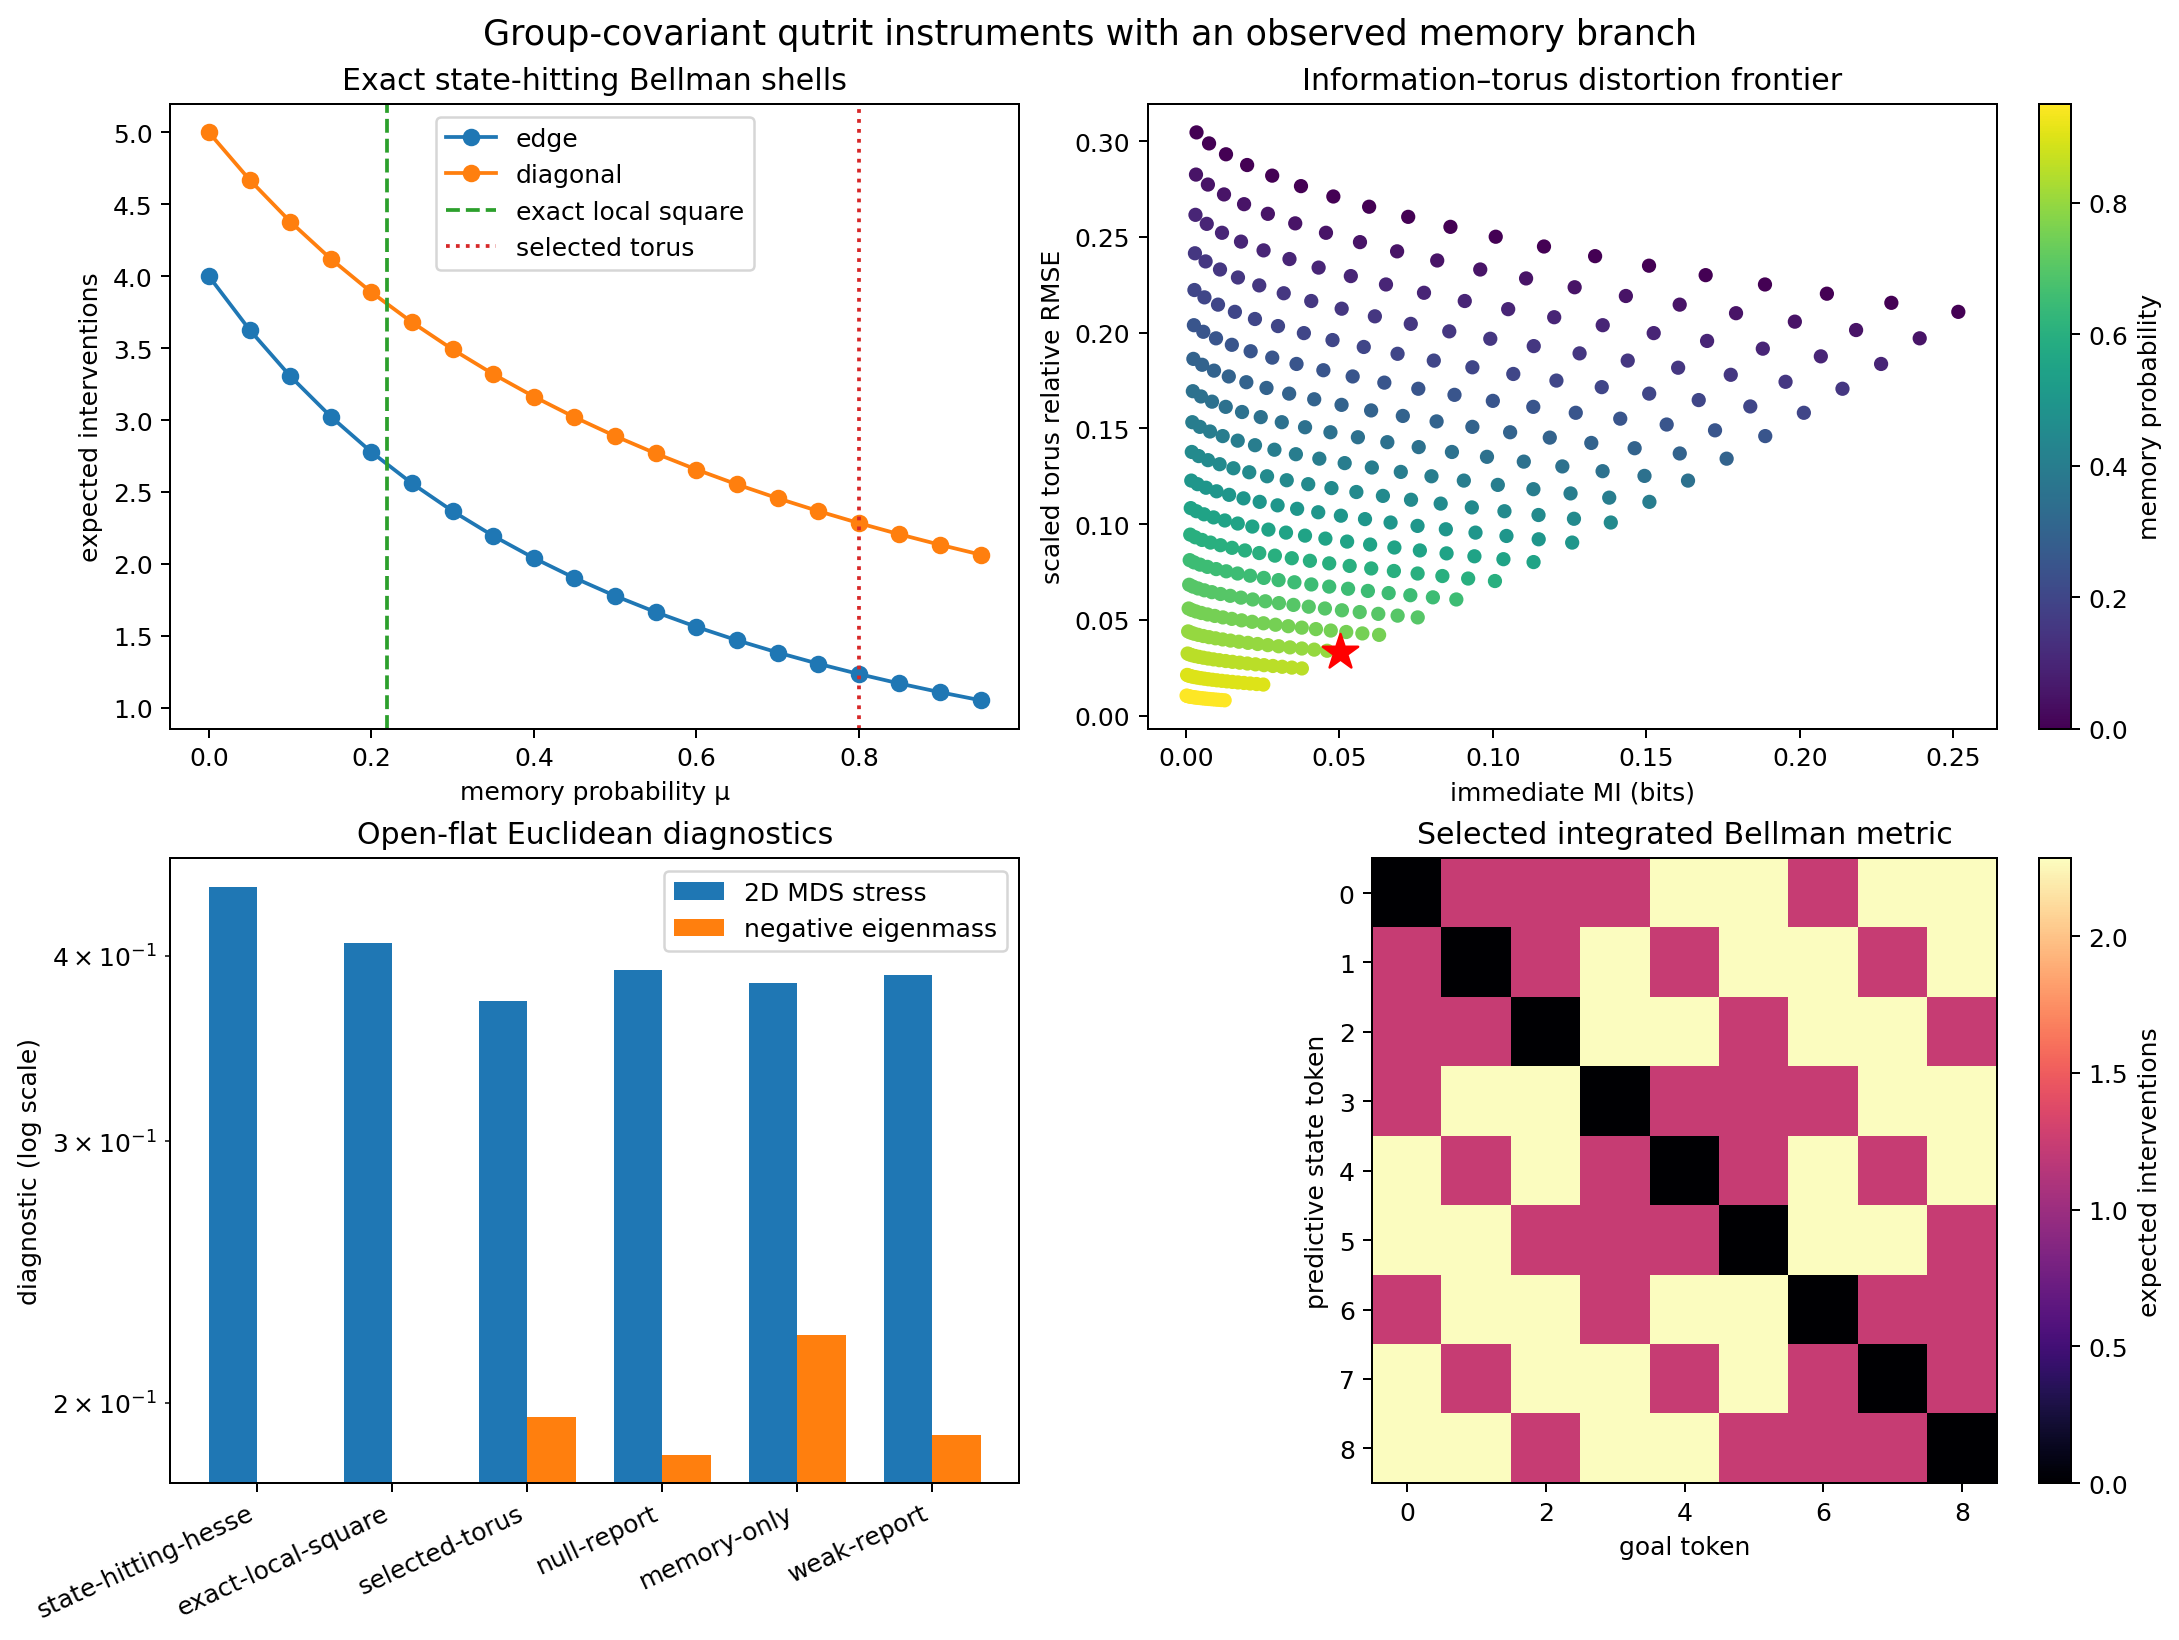
\includegraphics[width=\linewidth]{covariant_memory_search.png}
\caption{Exact covariant-memory search. Top left: analytic Bellman shells
across the sharp family, including the exact-square and selected values. Top
right: immediate information versus scaled torus distortion over all
\(380\) candidates. Bottom left: global embedding diagnostics prevent
local-square claims from being extended to a planar torus. Bottom right: the
selected all-pairs hitting metric.}
\label{fig:search}
\end{figure}

\subsection{Embedding and closure diagnostics}

The selected torus has negative Schoenberg eigenmass fraction \(0.1957\),
four positive centered dimensions, and two-dimensional MDS stress \(0.3731\).
The exact local-square cell has zero negative eigenmass and rank two, while its
full nine-token matrix has stress \(0.4082\). Correlation with an open
\(3\times3\) grid is only \(0.5276\), as expected from periodic boundaries.

All equal-length displacement classes through word length four close at
floating-point precision. The selected all-length trace-distance residual is
\(0.31866\). The Hesse reset endpoint is even more path-age sensitive
(\(0.66406\)); memory-only motion closes at numerical precision. These
numbers show length dependence of the outcome-discarded ensemble channel. They
do not establish a noise-age coordinate for the fully observing agent, whose
conditional branches close on pure Hesse rays.

\subsection{Finite-string validation}

With oracle-labelled Hesse source and successor classes, \(500\) trials per
state/action recovered all five memory-branch permutations. This is a
finite-state structural-identifiability audit, not opaque learning from the
instrument's emitted strings. A transition table trained on
\(400\) samples per pair was evaluated on \(2{,}000\) independent
length-eight strings:
\[
\begin{array}{lc}
\text{exact filter NLL}&1.3132\ {\rm bits/event},\\
\text{learned kernel NLL}&1.3989\ {\rm bits/event},\\
\text{state-marginal NLL}&3.8964\ {\rm bits/event}.
\end{array}
\]
The \(0.0857\)-bit oracle gap measures finite training error. The large
advantage over the marginal model shows that learned state and action meaning
generalize beyond one-step fitting.

\section{Opaque predictive learning}

\subsection{Experimental design}

The second experiment receives only shuffled action IDs and shuffled outcome
tokens. It receives no coordinates, density matrices, Kraus operators, or
displacement names. For each of six models, \(12{,}000\) training and
\(3{,}000\) held-out seven-step sequences were generated with seed
\(20260812\).

Three transparent predictors were fitted:
\begin{enumerate}
\item an action-only marginal model;
\item last outcome plus next action;
\item previous action/outcome, current outcome, and next action.
\end{enumerate}
The exact density-matrix filter is an oracle, not an input to learning.
Transition kernels were estimated from adjacent tokens; maximum-probability
maps were tested for bijectivity, orders, commutation, group size, and orbit.
Invalid nonbijective maps were assigned group order zero rather than being
misreported as a transformation group.

\subsection{Topology and Bellman recovery}

The rank-one baseline recovers five bijections: one identity and four
commuting order-three maps. They generate a transitive group of order nine.
Its learned state-hitting shells are approximately
\[
(0,3.9553,4.9232),
\]
near the exact \((0,4,5)\). Both Weyl-covariant Lüders models also recover a
bijective, commuting order-nine action group. Token-aggregated Bellman shells
are strictly ordered:
\[
\eta=0.55:\ (0,6.6285,7.0926),\qquad
\eta=0.80:\ (0,5.1137,5.9145).
\]
For these latent-memory models, token Bellman planning is an approximation
because the last token is not a sufficient causal state.

\begin{table}[H]
\centering
\caption{Held-out prediction and learned topology. NLL is bits per outcome.
The last column is the exact quantum-filter oracle.}
\label{tab:learning}
\begin{tabular}{lrrrrr}
\toprule
Model&Last token&Two-event&Oracle&Group&Orbit\\
\midrule
Rank-one reset&2.9568&2.9638&2.9549&9&9\\
Weyl Lüders \(\eta=.55\)&3.1491&3.1568&3.1137&9&9\\
Weyl Lüders \(\eta=.80\)&3.0740&3.0793&3.0172&9&9\\
Null Lüders&3.1734&3.1796&3.1699&0&1\\
Haar Lüders \(\eta=.55\)&3.1495&3.1581&3.1164&0&1\\
External-DFA null&3.1729&3.1803&3.1699&0&1\\
\bottomrule
\end{tabular}
\end{table}

\subsection{What prediction reveals about memory}

At \(\eta=0.55\), the last-token/oracle gap is \(0.03535\) bits per outcome;
at \(\eta=0.80\), it is \(0.05683\). The exact quantum filter uses information
that the last token discards. This is operational evidence of latent memory.

The naive two-event estimator did not exploit it: its held-out NLL was
slightly worse than last-token prediction. Raw future-law variation among
histories sharing a last token was comparable to the null sampling floor;
null-subtracted means were \(0.00093\) at \(\eta=.55\) and
\(-0.00134\) at \(\eta=.80\). It would be incorrect to call this noisy
suffix statistic a learned fiber. The oracle gap establishes that memory
exists; learning it requires a regularized PSR rather than context
proliferation.

\begin{figure}[H]
\centering
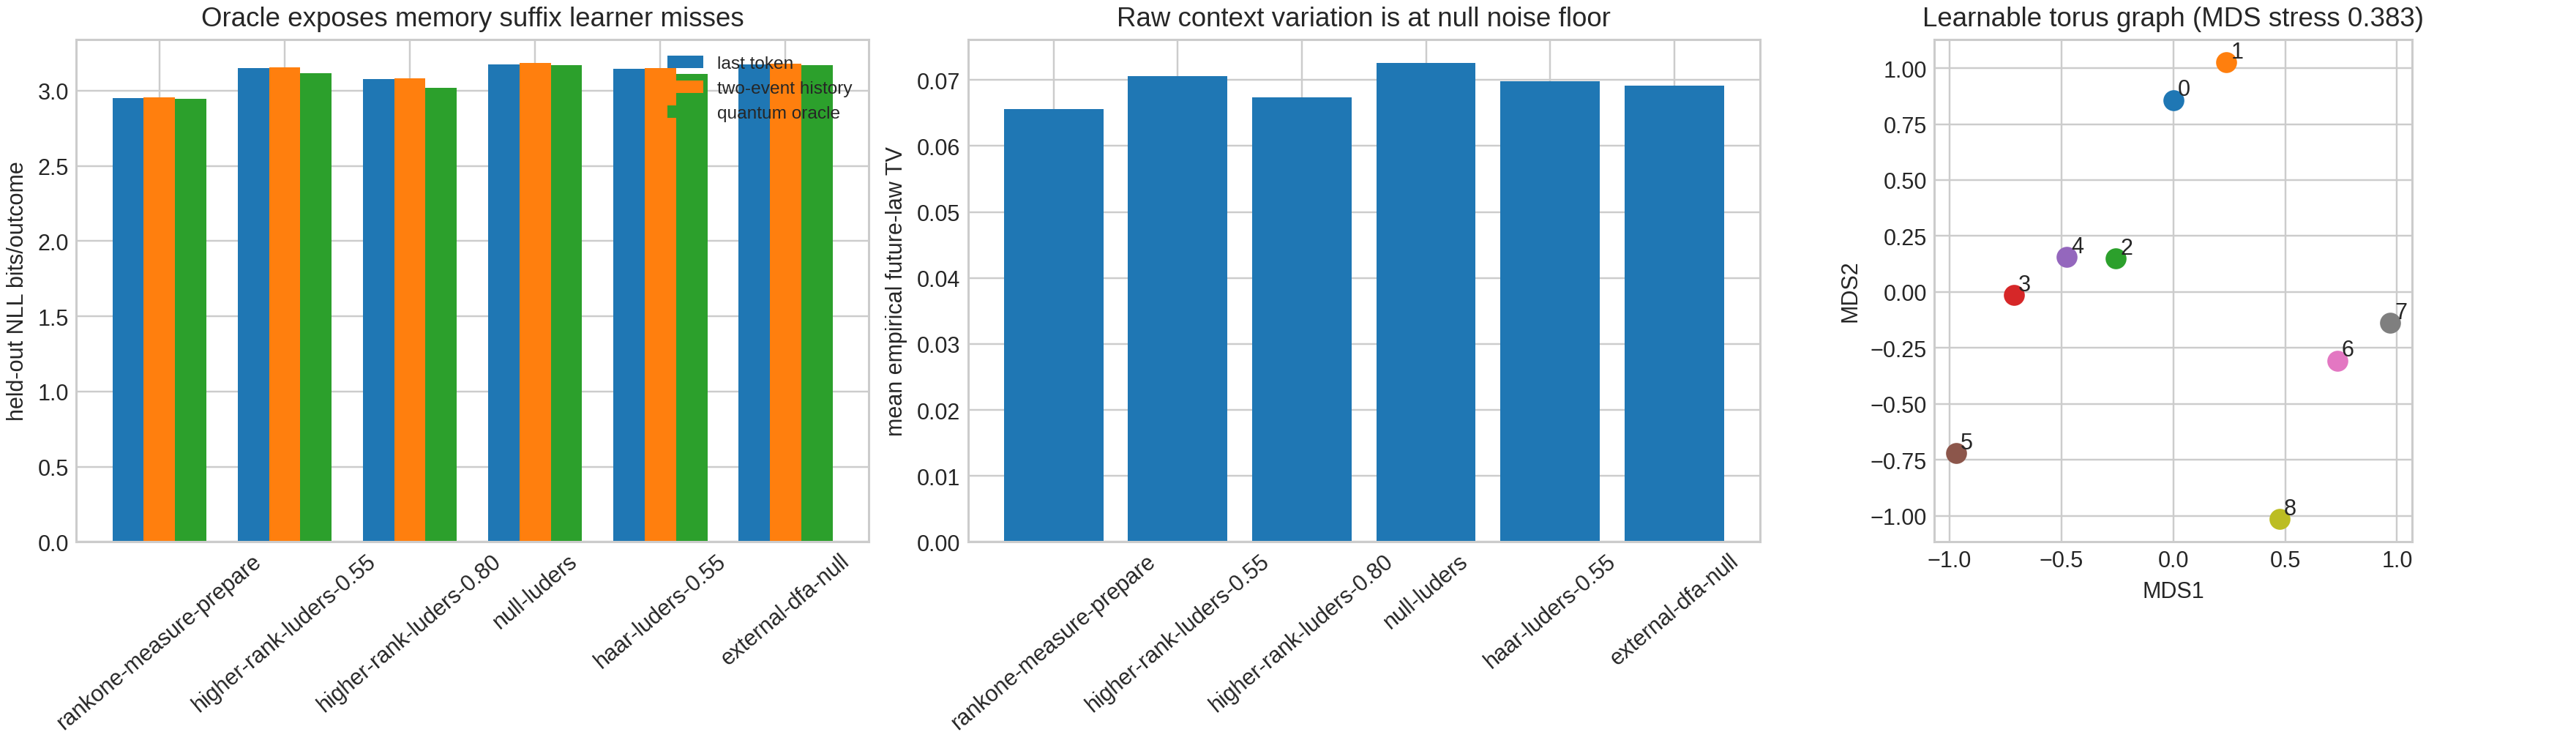
\includegraphics[width=\linewidth]{opaque_prediction_and_topology.png}
\caption{Opaque learning diagnostics. Left: exact quantum filtering exposes
predictive memory that a finite suffix model misses. Center: raw context
variation is at the null noise floor and is not claimed as learned memory.
Right: the learned torus graph is topologically correct, but its planar MDS
display has nonzero stress.}
\label{fig:opaque}
\end{figure}

\begin{figure}[H]
\centering
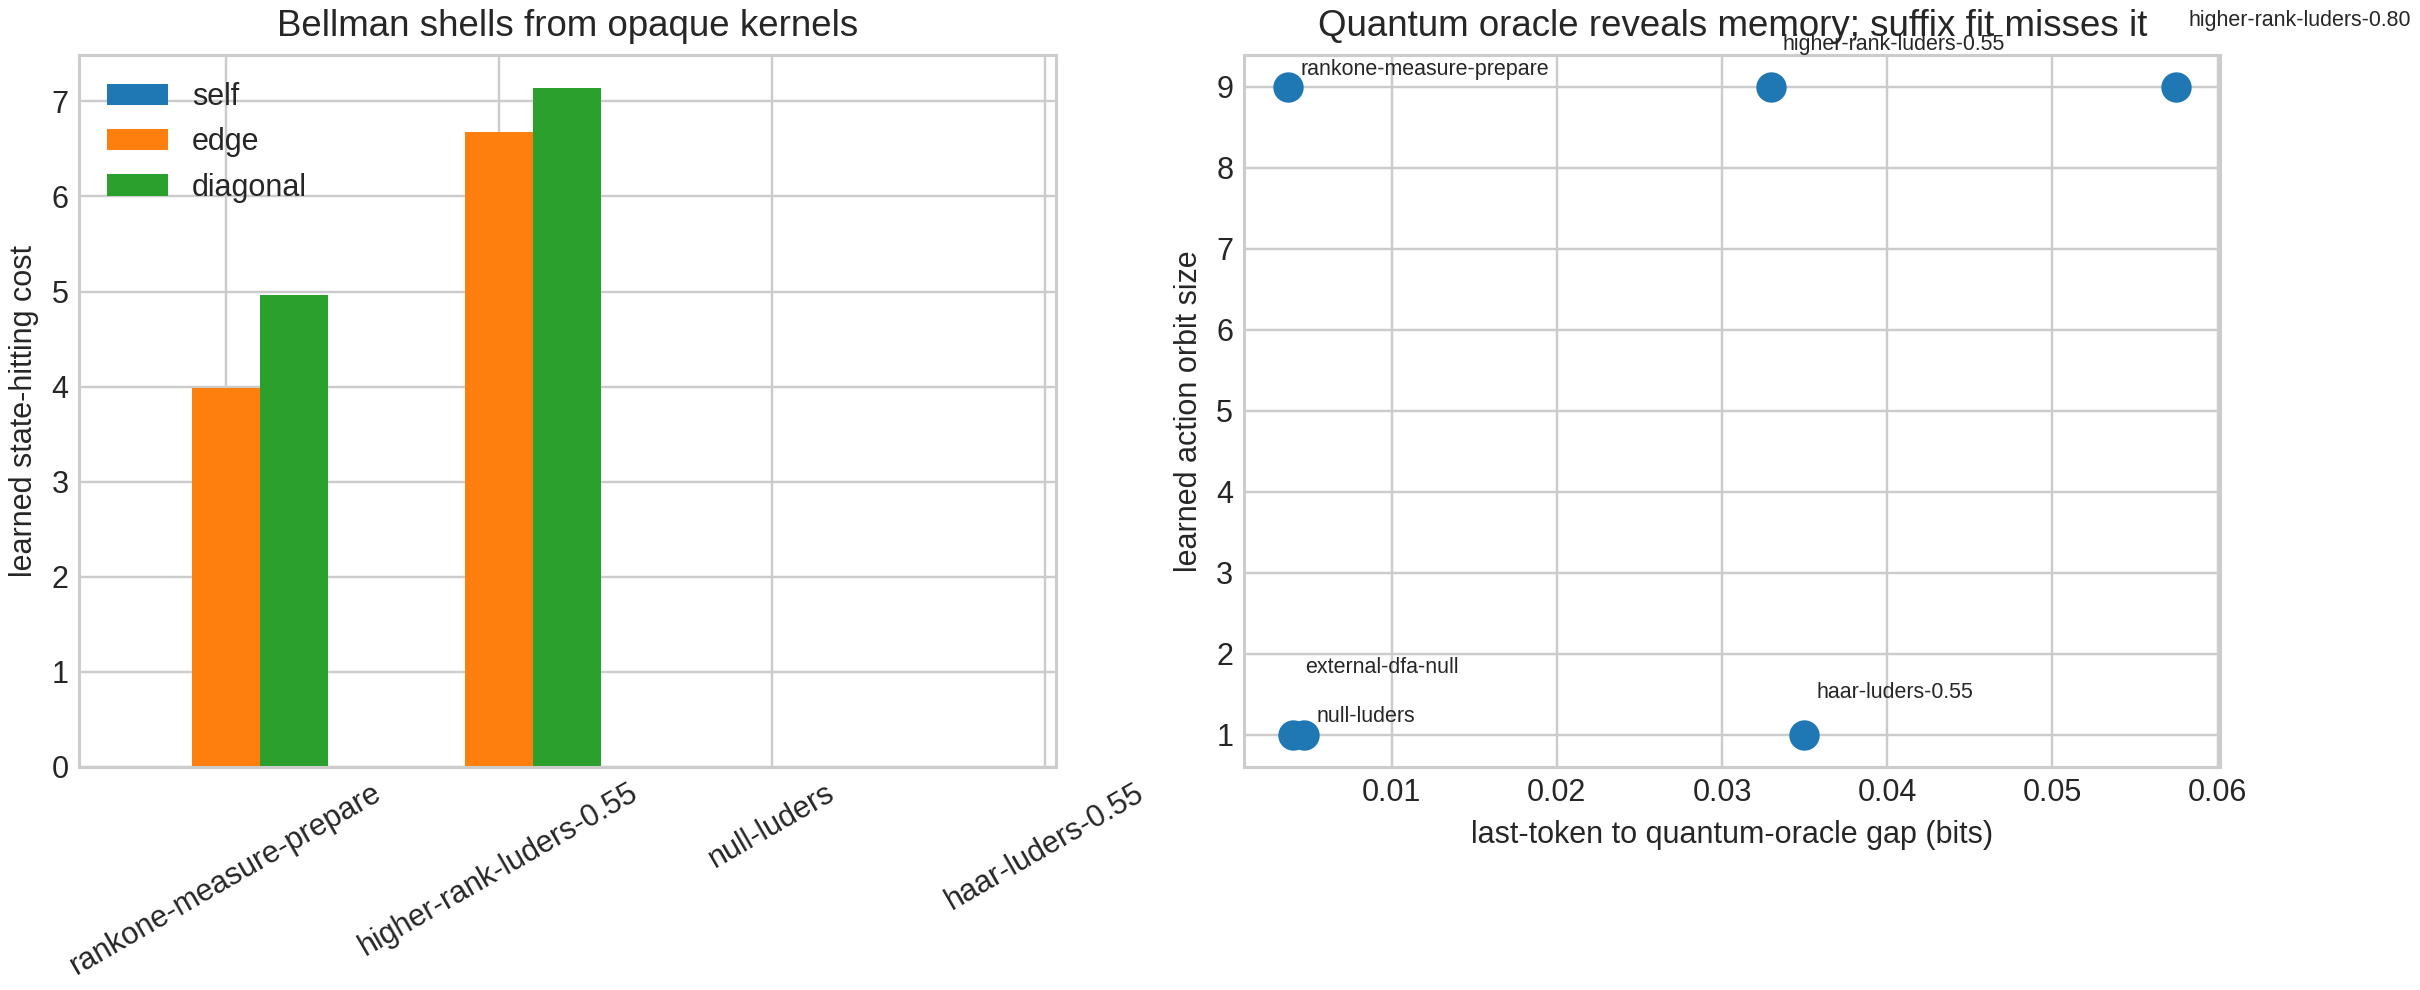
\includegraphics[width=.96\linewidth]{learned_bellman_and_controls.png}
\caption{Left: strict state-hitting shells recovered from opaque token
kernels. Right: spatial action topology and longer-history prediction are
independent tests. Null, Haar, and external-DFA controls fail bijective
translation-group recovery.}
\label{fig:controls}
\end{figure}

\subsection{Matched controls}

\begin{description}
\item[Rank-one Hesse reset.] Positive topology baseline with an exact
last-token predictive quotient but no retained branch.
\item[Null Lüders.] Uniform outcomes carry no state information and inferred
argmax maps are nonbijective.
\item[Haar Lüders.] Actions can affect future predictions but do not close
into the required commuting translation group.
\item[External DFA.] A nine-node classical counter has hand-coded goal
geometry while quantum outcomes remain null. The quantum predictive orbit is
one.
\item[Memory only.] The exact word metric \(0,1,2\) and perfect path closure
coexist with zero immediate information.
\item[Permutation gauge.] Persistent shuffling changes names, not group order,
commutation, orbit, or Bellman shells. Episode-wise reshuffling would destroy
persistent meaning.
\end{description}

\section{Information, disturbance, and geometry}

\subsection{Immediate information is not operational action meaning}

For a state label \(S\), outcome \(O\), and fixed action \(a\),
\[
I(S;O\mid A=a)=
\sum_{s,o}\pi_s p(o\mid s,a)
\log_2\frac{p(o\mid s,a)}
{\sum_t\pi_t p(o\mid t,a)}.
\]
This measures the current report. Future-operational action meaning instead
asks whether later test probabilities change. The memory-only endpoint has
zero immediate information but perfect future translation meaning. The null
instrument has neither. The Haar control has future meaning but the wrong
algebra. These examples separate three properties that a single mutual
information number cannot summarize.

Channel distinguishability may be quantified by the diamond norm
\(\|\Phi_a-\Phi_b\|_\diamond\), while future outcome distributions may use
total variation or Jensen--Shannon divergence \cite{Watrous2018}. These
measure distinguishability, not spatial covariance.

\subsection{No exact universal information without disturbance}

\begin{proposition}
If an instrument's nonselective channel equals a unitary channel
\(\cU(\rho)=U\rho U^\dagger\) on the full state space, then each branch is
\(\cE_o=p_o\cU\). Outcomes are input independent.
\end{proposition}
\begin{proof}
The Choi matrix of a unitary channel has rank one. Positive branch Choi
matrices sum to it, so every branch has support in that same one-dimensional
space: \(J(\cE_o)=p_oJ(\cU)\). The Choi isomorphism gives the result.
\end{proof}

The assumptions are exact and universal. Restricted commuting state families,
encoded subsystems, or approximate preservation allow information--disturbance
tradeoffs \cite{Holevo2011,Helstrom1976}. In this project, increasing reset
probability increases immediate information but also produces more
path-dependent noise.

\subsection{A base/fiber interpretation}

The learned permutations supply a base projection
\[
\pi:\mathcal S_{\rm predictive}\longrightarrow\Z_m^2.
\]
Predictive states with the same base token may differ in conditional density,
purity, path length, or uncertainty. Those residual degrees form a fiber
\(\mathcal F_x=\pi^{-1}(x)\). An action ideally has:
\begin{itemize}
\item a horizontal component translating \(x\);
\item a vertical/internal component evolving fiber state;
\item a coupling that may depend covariantly on the base.
\end{itemize}

Equation \cref{eq:path} makes a coarse-grained version concrete. Net
displacement determines the base, while \(\Phi^t\) records noise age only for
an observer who discards branch outcomes. A genuine predictive fiber appears
instead in the Lüders family, where histories with the same last token can
have different future laws; the oracle detects it, but the suffix learner does
not yet reconstruct it.

Operational holonomy can be studied from learned PSR action operators
\(B_a\). The loop
\[
\mathcal K_{ab}=B_aB_bB_a^{-1}B_b^{-1}
\]
transforms by similarity under PSR gauge. Its spectrum and future-test effect
are gauge invariant. Trivial base commutators with nontrivial fiber action
would provide a first operational analogue of a connection.

\section{What has and has not been established}

\subsection{Exact positive statements}

\begin{enumerate}
\item Correct state-hitting semantics converts the integrated Hesse result
from nonmetric \((4,4,5)\) to metric \((0,4,5)\).
\item The Hesse metric recovers a homogeneous \(\Z_3^2\) torus neighbor graph.
\item Its global Euclidean embedding dimension is exactly eight.
\item The observed memory/reset family is CPTP, covariant, informative for
\(\mu<1,\xi>0\), and exactly closed on nine predictive Hesse states.
\item Its Bellman shells have the closed forms
\cref{eq:general-shells,eq:sharp-shells}; strictness and triangles hold for
the entire sharp family.
\item The value \(\mu_\square\) gives exact Euclidean elementary squares.
\item Equal-length word closure follows analytically from covariance.
\end{enumerate}

\subsection{Numerical statements}

\begin{enumerate}
\item The constrained grid search selects a positive-information candidate
with \(3.33\%\) scaled torus distortion.
\item Oracle-labelled trials identify the exact family's finite action maps
and validate held-out length-eight tables; this is not opaque-string learning.
\item Opaque Lüders experiments recover a commuting order-nine group and
strict token-level hitting shells.
\item Exact quantum-filter likelihood exposes latent memory not captured by
the last token.
\item Null, Haar, and external-memory controls fail at their predicted
operational layer.
\end{enumerate}

\subsection{Limitations}

\begin{enumerate}
\item Equal displacement does not imply equal predictive state across
different path lengths. The selected all-length residual is \(0.319\).
\item A \(3\times3\) torus is not an open planar \(3\times3\) grid. Only the
elementary four-state square is exactly planar in the present construction.
\item The observed memory/reset outcome grammar is engineered. It has not
emerged from unconstrained instrument optimization.
\item The suffix learner does not recover the latent fiber. The oracle
demonstrates its existence, not its learned representation.
\item Token-aggregated Bellman values for Lüders models are approximations to
belief-state values.
\item Immediate information, metric quality, and memory retention are
multiobjective; no canonical scalar weighting has been justified.
\item Finite torus graph distance is locally Manhattan. Calling it Riemannian
would overstate the result.
\end{enumerate}

\section{Future research}

\subsection{Larger phase tori and honest flat patches}

A qutrit supports arbitrarily many nonorthogonal phase landmarks:
\[
|\phi_{xy}^{(m)}\rangle=
\frac{|0\rangle+\zeta^x|1\rangle+\zeta^y|2\rangle}{\sqrt3},
\qquad \zeta=e^{2\pi i/m},
\]
with commuting controls
\[
U_x=\operatorname{diag}(1,\zeta,1),\qquad
U_y=\operatorname{diag}(1,1,\zeta).
\]
For \(m=5,7,9\), nonwrapping patches of radius \(r<m/2\) contain multiple
plaquettes. A covariant phase POVM and positive Choi seed can then be
optimized for information, strict hitting costs, local isotropy, and weak
fiber disturbance.

\subsection{Spectral PSRs}

Suffix tables proliferate contexts and performed worse at the available
sample size. The next learner should:
\begin{enumerate}
\item collect controlled history/test Hankel blocks over increasing horizons;
\item select rank with bootstrap singular-value intervals and held-out
shrinkage;
\item fit low-rank action/outcome update operators;
\item test shifted-Hankel action separation and group relations in PSR gauge;
\item solve goal problems in learned predictive state rather than last-token
state;
\item compare with the exact quantum filter only as a calibration oracle.
\end{enumerate}
Spectral PSRs expose rank and linear gauge explicitly
\cite{Littman2001,Hsu2012}. Recurrent models can follow after the transparent
baseline.

\subsection{Instrument optimization}

Use \cref{prop:choi} with \(C_0=LL^\dagger\), enforcing covariance and CPTP
exactly. Optimize a Pareto frontier rather than one opaque loss:
\[
\max\{I_{\rm immediate},I_{\rm future},M,\Delta_{\rm edge}\},\qquad
\min\{1-F_{\rm move},\epsilon_{\rm path},\epsilon_{\rm flat}\}.
\]
Here \(M\) is same-outcome future separation, \(F_{\rm move}\) is fidelity to
the intended unitary move, and \(\epsilon_{\rm flat}\) measures translated
patch inconsistency. Search should begin from the observed and two-Kraus
analytic families before allowing an unrestricted Choi seed.

\subsection{Toward bundles and curvature}

The spatial base should be the coarsest predictive quotient preserving
place-like goal values and local action increments. Posterior uncertainty,
measurement context, goal progress, and quantum memory remain in the fiber.
Loop transformations can probe connection and curvature. Eventually,
state-dependent local cost tensors and nontrivial holonomy could connect
hodological geometry to dynamical spacetime models. At the present stage,
these are research directions, not conclusions.

\section{Conclusion}

A qutrit is large enough to support an operationally learned two-dimensional
translation topology and a strict goal metric without nine orthogonal basis
states. The key correction is conceptual: being at a goal and being required
to report it again are different reinforcement-learning tasks. Standard
state-hitting semantics gives the exact integrated Hesse metric
\((0,4,5)\).

Retained memory then supplies a controlled interpolation. The observed
memory/reset family joins positive immediate information, exact finite
conditional states, covariant translations, and analytic Bellman geometry.
One parameter value gives exact local squares; another gives a high-memory
torus approximation selected by a transparent rule. Oracle-labelled trials
verify its finite maps, while a separate opaque Lüders experiment recovers the
torus action group from emitted strings.

The Lüders oracle gap identifies latent predictive memory over the spatial
token base, but the present learner does not yet reconstruct that candidate
fiber. The next decisive step is to learn it with a spectral PSR on a larger torus and
test translated nonwrapping patches. Geometry should be claimed only after
prediction, action algebra, Bellman metricity, topology, and local embedding
all pass separate controls.

\appendix
\section{Reproducibility and acceptance criteria}

\subsection{Commands and artifacts}

From the search directory, run the seven focused unit tests and deterministic
search:
\begin{verbatim}
python -m unittest discover -s tests -v
MPLBACKEND=Agg python run_search.py
\end{verbatim}
From the learning directory:
\begin{verbatim}
python -m unittest -v test_opaque_learning.py
MPLBACKEND=Agg python opaque_learning.py --train 12000 \
  --test 3000 --seed 20260812
\end{verbatim}

The search archive contains all \(380\) grid points, candidate diagnostics,
path closure tables, all-pairs Bellman matrices, a JSON manifest, and
\cref{fig:search}. The learning archive contains summary and action-algebra
tables, per-model transition kernels, Hankel singular spectra, a manifest, and
\cref{fig:opaque,fig:controls}.

\subsection{Acceptance table}

\begin{longtable}{p{.18\linewidth}p{.34\linewidth}p{.37\linewidth}}
\caption{Preregistered-style criteria for a future covariant-memory geometry.}
\label{tab:accept}\\
\toprule
Layer&Statistic&Acceptance\\
\midrule
\endfirsthead
\toprule
Layer&Statistic&Acceptance\\
\midrule
\endhead
Physical&Kraus completeness and covariance residual&Below \(10^{-10}\)\\
Prediction&Held-out NLL and calibration&Better than matched marginal/null\\
Memory&Same-outcome future separation&Bootstrap interval above zero\\
Action&Shifted-Hankel pair separation&Every intended distinct pair\\
Algebra&Orders, commutators, orbit&\(\Z_m^2\) within uncertainty\\
Hitting&Bellman solution&Finite; residual below \(10^{-10}\)\\
Metric&Strictness, symmetry, triangles&No significant violations\\
Topology&Lowest-cost neighbor graph&Torus isomorphism\\
Local geometry&Patch residual and increment variance&Stable below declared threshold\\
Controls&Null, cloned, Haar, DFA tests&Fail at predicted layer\\
\bottomrule
\end{longtable}

\section{Derivation audit for the sharp family}

Substituting \(\xi=1\) in \cref{eq:general-bellman} gives
\[
c=\frac{1-\mu}{3},\quad
h=\mu+\frac{7(1-\mu)}{12}=\frac{7+5\mu}{12},\quad
A=\frac{2+\mu}{3}.
\]
Then
\[
A^2-ch
=\frac{(2+\mu)^2}{9}
-\frac{(1-\mu)(7+5\mu)}{36}
=\frac{(1+\mu)^2}{4},
\]
which yields \(E=4/(1+\mu)^2\). Further,
\[
D=\frac{1+hE}{A}
=\frac{3\mu+5}{(1+\mu)^2}.
\]
At \(\mu=0\), these reproduce \cref{thm:hesse}; at \(\mu=1\), deterministic
memory motion yields one cardinal step or two.

\begin{thebibliography}{99}

\bibitem{Kraus1983}
K.~Kraus,
\emph{States, Effects, and Operations: Fundamental Notions of Quantum
Theory}, Springer, Berlin (1983).

\bibitem{NielsenChuang2010}
M.~A. Nielsen and I.~L. Chuang,
\emph{Quantum Computation and Quantum Information}, 10th anniversary ed.,
Cambridge University Press, Cambridge (2010).

\bibitem{Renes2004}
J.~M. Renes, R.~Blume-Kohout, A.~J. Scott, and C.~M. Caves,
Symmetric informationally complete quantum measurements,
\emph{Journal of Mathematical Physics} \textbf{45}, 2171--2180 (2004).

\bibitem{Littman2001}
M.~L. Littman, R.~S. Sutton, and S.~Singh,
Predictive representations of state,
\emph{Advances in Neural Information Processing Systems} \textbf{14} (2001).

\bibitem{Hsu2012}
D.~Hsu, S.~M. Kakade, and T.~Zhang,
A spectral algorithm for learning hidden Markov models,
\emph{Journal of Computer and System Sciences} \textbf{78}, 1460--1480
(2012).

\bibitem{NielsenGST2020}
E.~Nielsen, J.~K. Gamble, K.~Rudinger, T.~Scholten, K.~Young, and
R.~Blume-Kohout,
Gate set tomography,
arXiv:2009.07301 (2020).

\bibitem{DiMatteo2020}
O.~Di Matteo, J.~Gamble, C.~Granade, K.~Rudinger, and N.~Wiebe,
Operational, gauge-free quantum tomography,
arXiv:2007.01470 (2020).

\bibitem{SuttonBarto2018}
R.~S. Sutton and A.~G. Barto,
\emph{Reinforcement Learning: An Introduction}, 2nd ed.,
MIT Press, Cambridge, MA (2018).

\bibitem{Puterman1994}
M.~L. Puterman,
\emph{Markov Decision Processes: Discrete Stochastic Dynamic Programming},
Wiley, New York (1994).

\bibitem{Schoenberg1935}
I.~J. Schoenberg,
Remarks to Maurice Fr\'echet's article on axiomatically defined distance
spaces,
\emph{Annals of Mathematics} \textbf{36}, 724--732 (1935).

\bibitem{BorgGroenen2005}
I.~Borg and P.~J.~F. Groenen,
\emph{Modern Multidimensional Scaling: Theory and Applications}, 2nd ed.,
Springer, New York (2005).

\bibitem{Watrous2018}
J.~Watrous,
\emph{The Theory of Quantum Information},
Cambridge University Press, Cambridge (2018).

\bibitem{Holevo2011}
A.~S. Holevo,
\emph{Probabilistic and Statistical Aspects of Quantum Theory},
Edizioni della Normale, Pisa (2011).

\bibitem{Helstrom1976}
C.~W. Helstrom,
\emph{Quantum Detection and Estimation Theory},
Academic Press, New York (1976).

\end{thebibliography}
\end{document}
